\PassOptionsToPackage{unicode=true}{hyperref} % options for packages loaded elsewhere
\PassOptionsToPackage{hyphens}{url}
%
\documentclass[10pt,xcolor=table,color={dvipsnames,usenames},ignorenonframetext,usepdftitle=false,french]{beamer}
\setbeamertemplate{caption}[numbered]
\setbeamertemplate{caption label separator}{: }
\setbeamercolor{caption name}{fg=normal text.fg}
\beamertemplatenavigationsymbolsempty
\usepackage{caption}
\captionsetup{skip=0pt,belowskip=0pt}
%\setlength\abovecaptionskip{-15pt}
\usepackage{lmodern}
\usepackage{amssymb,amsmath,mathtools,multirow}
\usepackage{float,hhline}
\usepackage{tikz}
\usepackage[tikz]{bclogo}
\usepackage{mathtools}
\usepackage{ifxetex,ifluatex}
\usepackage{fixltx2e} % provides \textsubscript
\ifnum 0\ifxetex 1\fi\ifluatex 1\fi=0 % if pdftex
  \usepackage[T1]{fontenc}
  \usepackage[utf8]{inputenc}
  \usepackage{textcomp} % provides euro and other symbols
\else % if luatex or xelatex
  \usepackage{unicode-math}
  \defaultfontfeatures{Ligatures=TeX,Scale=MatchLowercase}
\fi
\usetheme[coding=utf8,language=french,
,titlepagelogo=img/SACElogo.jpg
]{TorinoTh}
% use upquote if available, for straight quotes in verbatim environments
\IfFileExists{upquote.sty}{\usepackage{upquote}}{}
% use microtype if available
\IfFileExists{microtype.sty}{%
\usepackage[]{microtype}
\UseMicrotypeSet[protrusion]{basicmath} % disable protrusion for tt fonts
}{}
\IfFileExists{parskip.sty}{%
\usepackage{parskip}
}{% else
\setlength{\parindent}{0pt}
\setlength{\parskip}{6pt plus 2pt minus 1pt}
}
\usepackage{hyperref}
\hypersetup{
            pdftitle={Du bon usage des modèles Reg-ARIMA en désaisonnalisation},
            pdfauthor={Dominique Ladiray et Alain Quartier-la-Tente},
            pdfborder={0 0 0},
            breaklinks=true}
\urlstyle{same}  % don't use monospace font for urls
\newif\ifbibliography
\usepackage{graphicx,grffile}
\makeatletter
\def\maxwidth{\ifdim\Gin@nat@width>\linewidth\linewidth\else\Gin@nat@width\fi}
\def\maxheight{\ifdim\Gin@nat@height>\textheight\textheight\else\Gin@nat@height\fi}
\makeatother
% Scale images if necessary, so that they will not overflow the page
% margins by default, and it is still possible to overwrite the defaults
% using explicit options in \includegraphics[width, height, ...]{}
\setkeys{Gin}{width=\maxwidth,height=\maxheight,keepaspectratio}
% Prevent slide breaks in the middle of a paragraph:
\widowpenalties 1 10000
\raggedbottom
\AtBeginPart{
  \let\insertpartnumber\relax
  \let\partname\relax
  \frame{\partpage}
}
\AtBeginSection{
  \ifbibliography
  \else
    \begin{frame}{Sommaire}
    \tableofcontents[currentsection, hideothersubsections]
    \end{frame}
  \fi
}
\setlength{\emergencystretch}{3em}  % prevent overfull lines
\providecommand{\tightlist}{%
  %\setlength{\itemsep}{0pt}
  \setlength{\parskip}{0pt}
  }
\setcounter{secnumdepth}{0}

% set default figure placement to htbp
\makeatletter
\def\fps@figure{htbp}
\makeatother

\usepackage{booktabs}
\usepackage{longtable}
\usepackage{array}
\usepackage{multirow}
\usepackage[table]{xcolor}
\usepackage{wrapfig}
\usepackage{float}
\usepackage{colortbl}
\usepackage{pdflscape}
\usepackage{tabu}
\usepackage{threeparttable}
\usepackage{threeparttablex}
\usepackage[normalem]{ulem}
\usepackage{makecell}

\title{Du bon usage des modèles Reg-ARIMA en désaisonnalisation}
\ateneo{Journées de méthodologie statistique (JMS) - 2018}
\author{Dominique Ladiray et Alain Quartier-la-Tente}
\date{}


\setrellabel{}

\setcandidatelabel{}

\rel{}
\division{Département des Méthodes Statistiques}

\departement{Insee, Seasonal Adjustment Centre of Excellence (SACE)}
\makeatletter
\let\@@magyar@captionfix\relax
\makeatother

\DeclareMathOperator{\Cov}{Cov}
\newcommand{\E}[1]{\mathbb{E}\left[ #1 \right]}
\newcommand{\V}[1]{\mathbb{V}\left[ #1 \right]}
\newcommand{\cov}[2]{\Cov\left( #1\,,\,#2 \right)}

\begin{document}
\frame[plain,noframenumbering]{\titlepage}

\begin{frame}{Introduction à la procédure de désaisonnalisation}

\centering
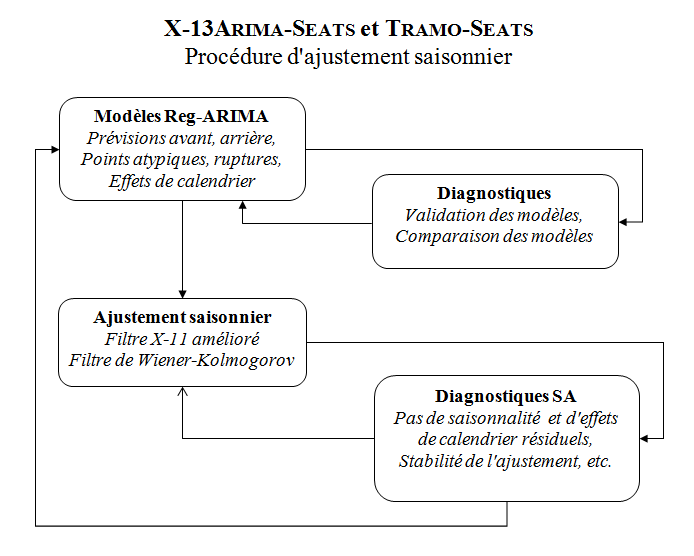
\includegraphics[height = 0.9\textheight]{img/MethodesX13-TS.png}

\end{frame}

\begin{frame}{Écriture mathématique du Reg-ARIMA}

Écriture mathématique du modèle Reg-ARIMA en désaisonnalisation :

\[
 \begin{drcases}
\text{Additif : }& Y_t \\
\text{Multiplicatif : }& \log(Y_t) 
\end{drcases} 
= \underbrace{\beta_0 LY_t + \beta_1 WD_t}_{\text{Régresseurs JO}} + 
\underbrace{\sum_{i}\gamma_iO_{i,t}}_{\mathclap{\text{Ruptures}}} + \underbrace{\varepsilon_t}_{\sim ARIMA}
\]

\medskip

\pause
Objectif de l'étude : illustrer des problèmes d'instabilité des
estimations avec des exemples sur :

\begin{itemize}
\item
  la correction de l'effet année bissextile (\emph{leap year})
\item
  l'estimation de ruptures (\emph{outliers})
\item
  l'identification du modèle ARIMA
\end{itemize}

\end{frame}

\section{Correction de l'effet année
bissextile}\label{correction-de-leffet-annee-bissextile}

\subsection{Quand et comment corriger l'effet année bissextile
?}\label{quand-et-comment-corriger-leffet-annee-bissextile}

\begin{frame}{Quand faut-il le corriger ?}

Année bissextile (\emph{leap year}) : un jour en plus en février
\(\simeq\) 4 ans

\(\rightarrow\) prise en compte de l'effet «~longueur du mois~» : c'est
un effet de calendrier

\medskip

Quand le corriger \bcquestion 

\medskip \pause

D'après les \emph{guidelines} sur l'ajustement saisonnier, le faire
lorsque :

\begin{itemize}
\item
  il y a un sens économique à le faire
\item
  l'effet est stable et statistiquement significatif
\end{itemize}

\medskip \pause
Étude des IPI européens (1330 séries) : l'effet \emph{leap year} existe
(mais pas toujours mesurable du fait de la collecte)

\end{frame}

\begin{frame}{Deux méthodes pour le corriger}

\begin{enumerate}
\item<1-> Avec le modèle Reg-ARIMA
\[
LY_t = \begin{cases}
0,75 & \text{ si $t$ est un mois de février bissextil} \\
-0,25  & \text{ si $t$ est un mois de février non bissextil} \\
0 & \text{ sinon}
\end{cases}
\]
\item<2-> Avec une correction \emph{a priori} en multipliant la série initiale par : 
\[\begin{cases}
\frac{28,25}{29} \simeq 0,974 & \text{ mois de février bissextil} \\
\frac{28,25}{28} \simeq 1,009 & \text{ mois de février non bissextil} \\
1 & \text{ sinon}
\end{cases}
\]
\end{enumerate}

\pause[3]

{[}Bell, 1992{]} : les deux méthodes équivalentes si schéma
multiplicatif et valeur estimée proche de 0,035
(\(\simeq \frac{29}{28}-1\), valeur attendue)

\pause[4]

\(\rightarrow\) Étude des estimations de la 1\iere{} méthode

\end{frame}

\subsection{Méthodologie de l'étude}\label{methodologie-de-letude}

\begin{frame}{Méthodologie utilisée}

Méthodologie : modèle \highlightbf{identifié} sur l'ensemble de la
période (ARIMA, outliers, etc.) et estimation mois par mois sur le passé
en \highlightbf{figeant} la date de début d'estimation

\pause
\medskip
On considère qu'il y a convergence lorsque le coefficient estimé reste :

\begin{itemize}
\item
  positif
\item
  non significativement différent de la dernière valeur
\item
  significative : stabilité du choix de corriger
\end{itemize}

\(\implies\) IPI européen : 410 séries convergent

\end{frame}

\subsection{Exemples}\label{exemples}

\begin{frame}{Exemples (1/2) : IPI FR-0610 (extraction de pétrole brut)}

\centering
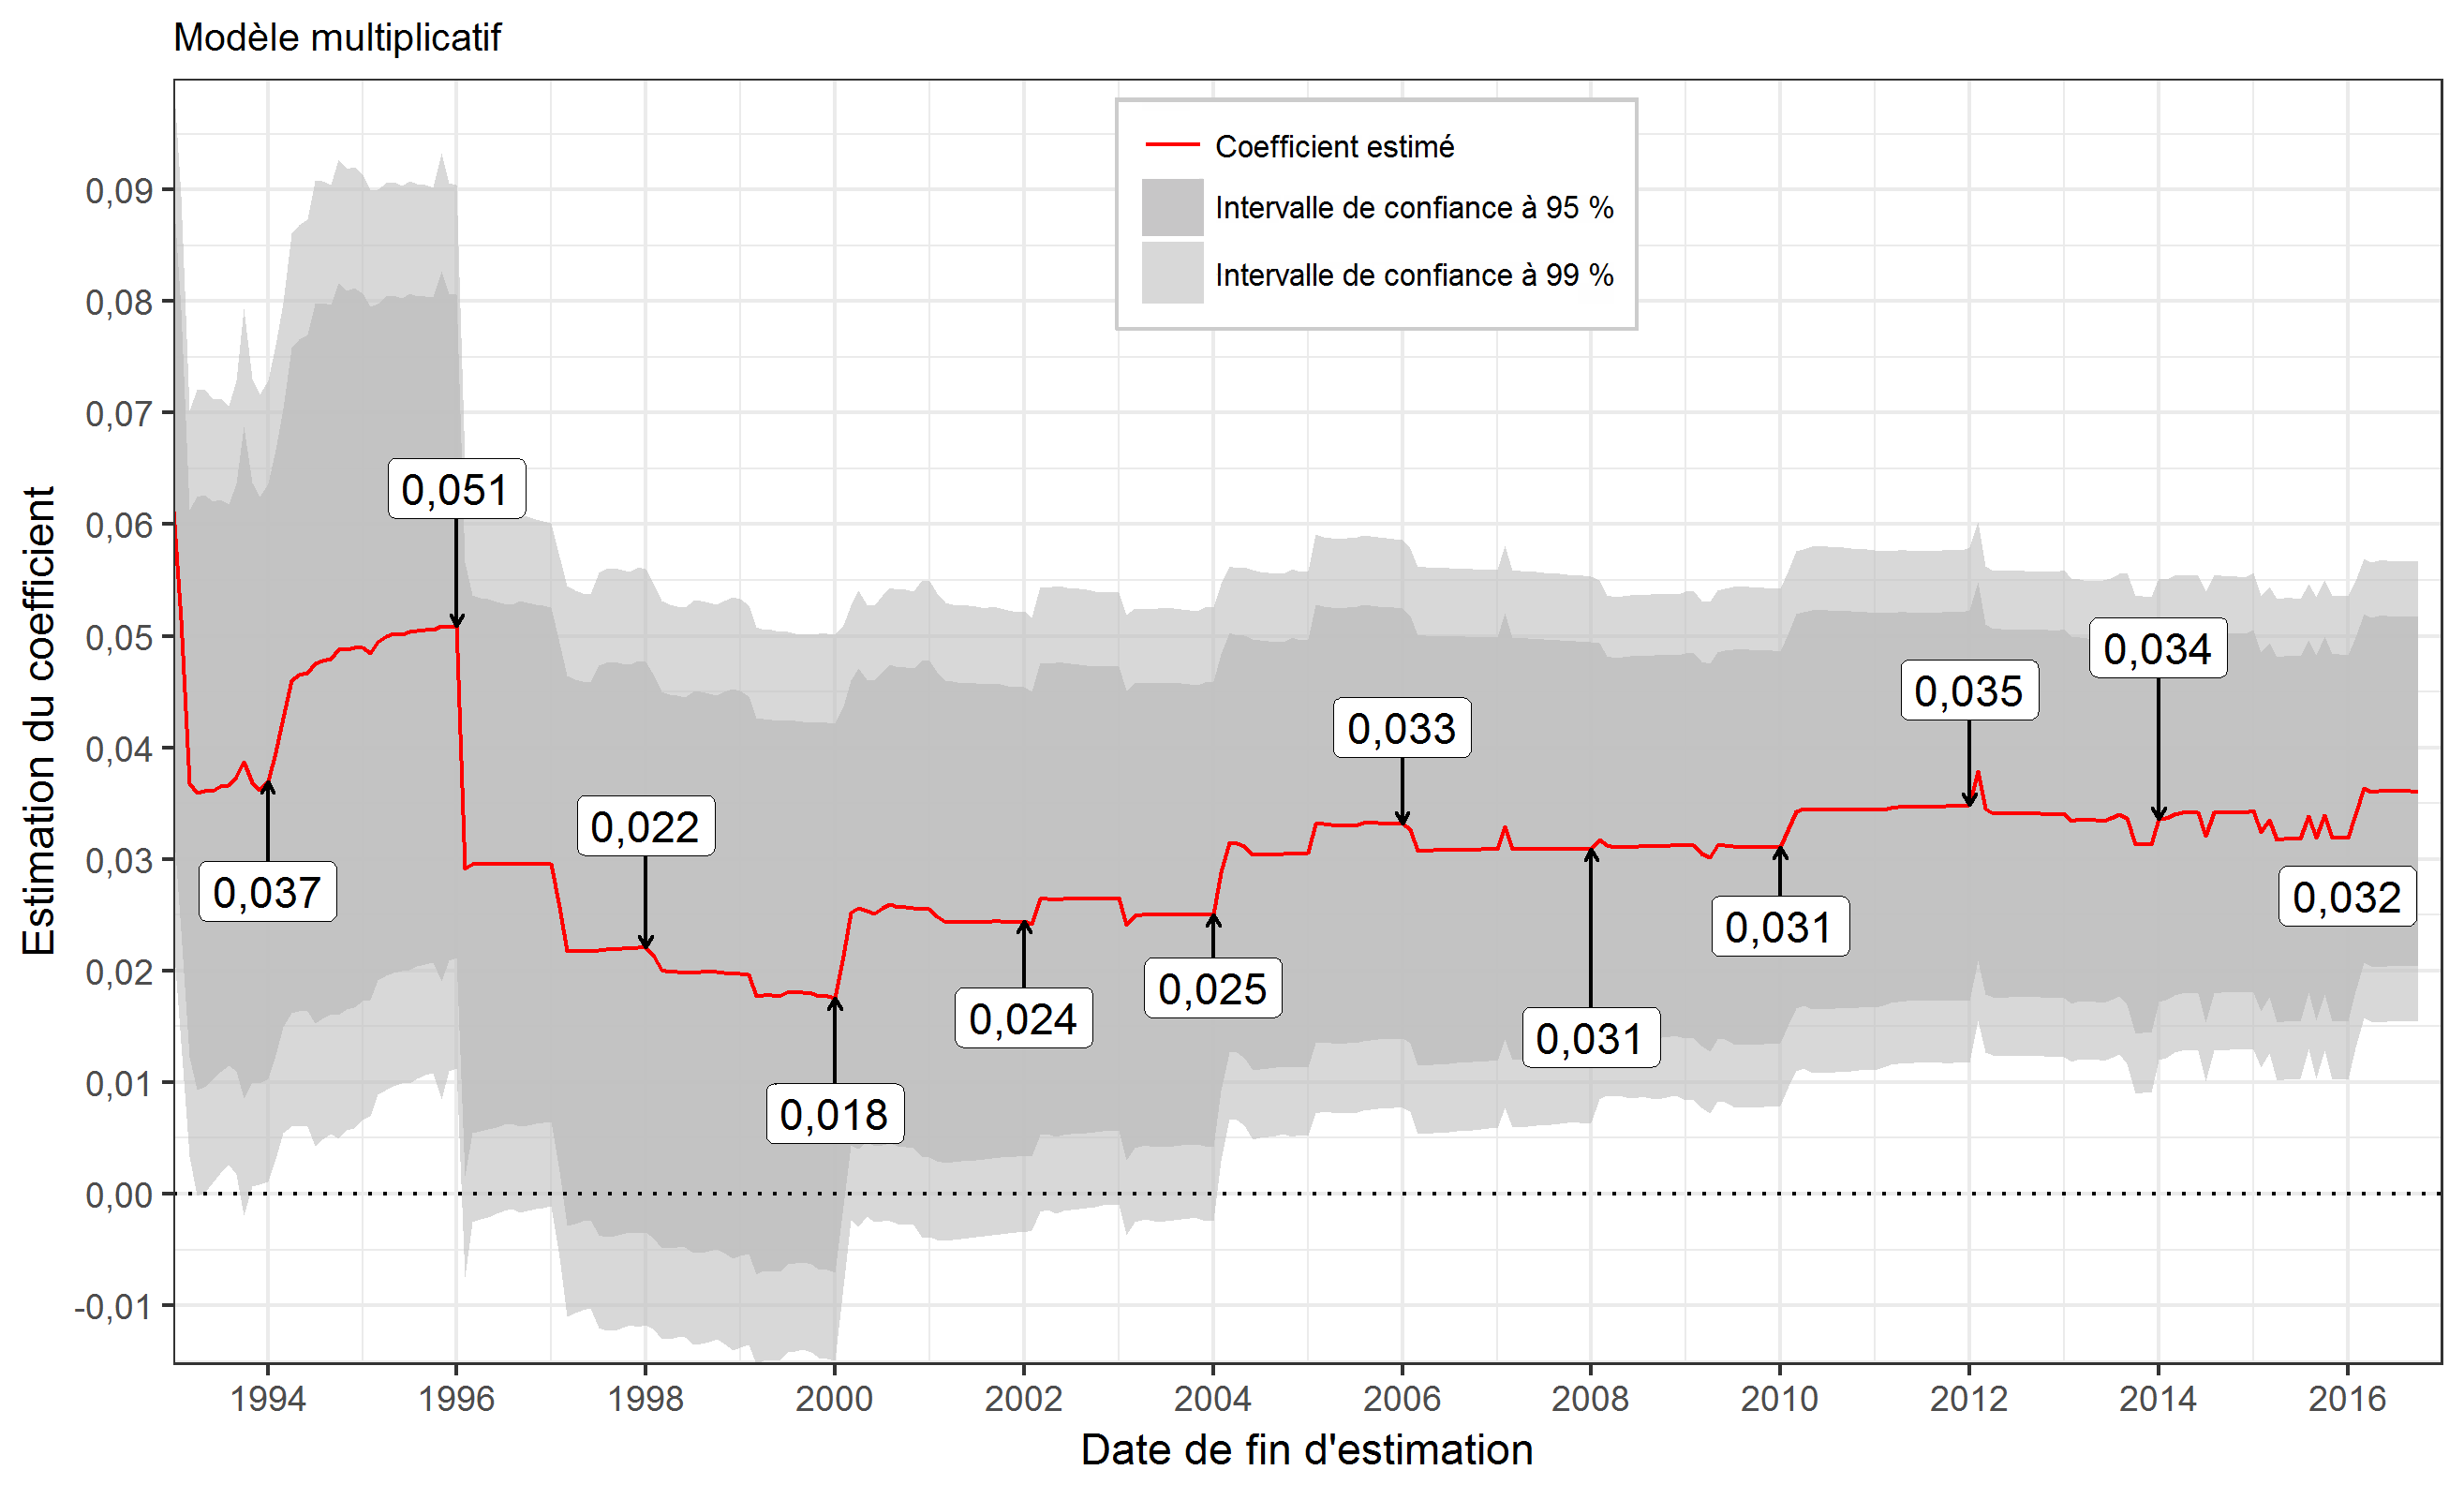
\includegraphics[width = \textwidth]{img/LYexemple1.png}

\end{frame}

\begin{frame}{Exemples (2/2) : IPI FR-1391 (Fabrication d'étoffes à
mailles)}

\centering
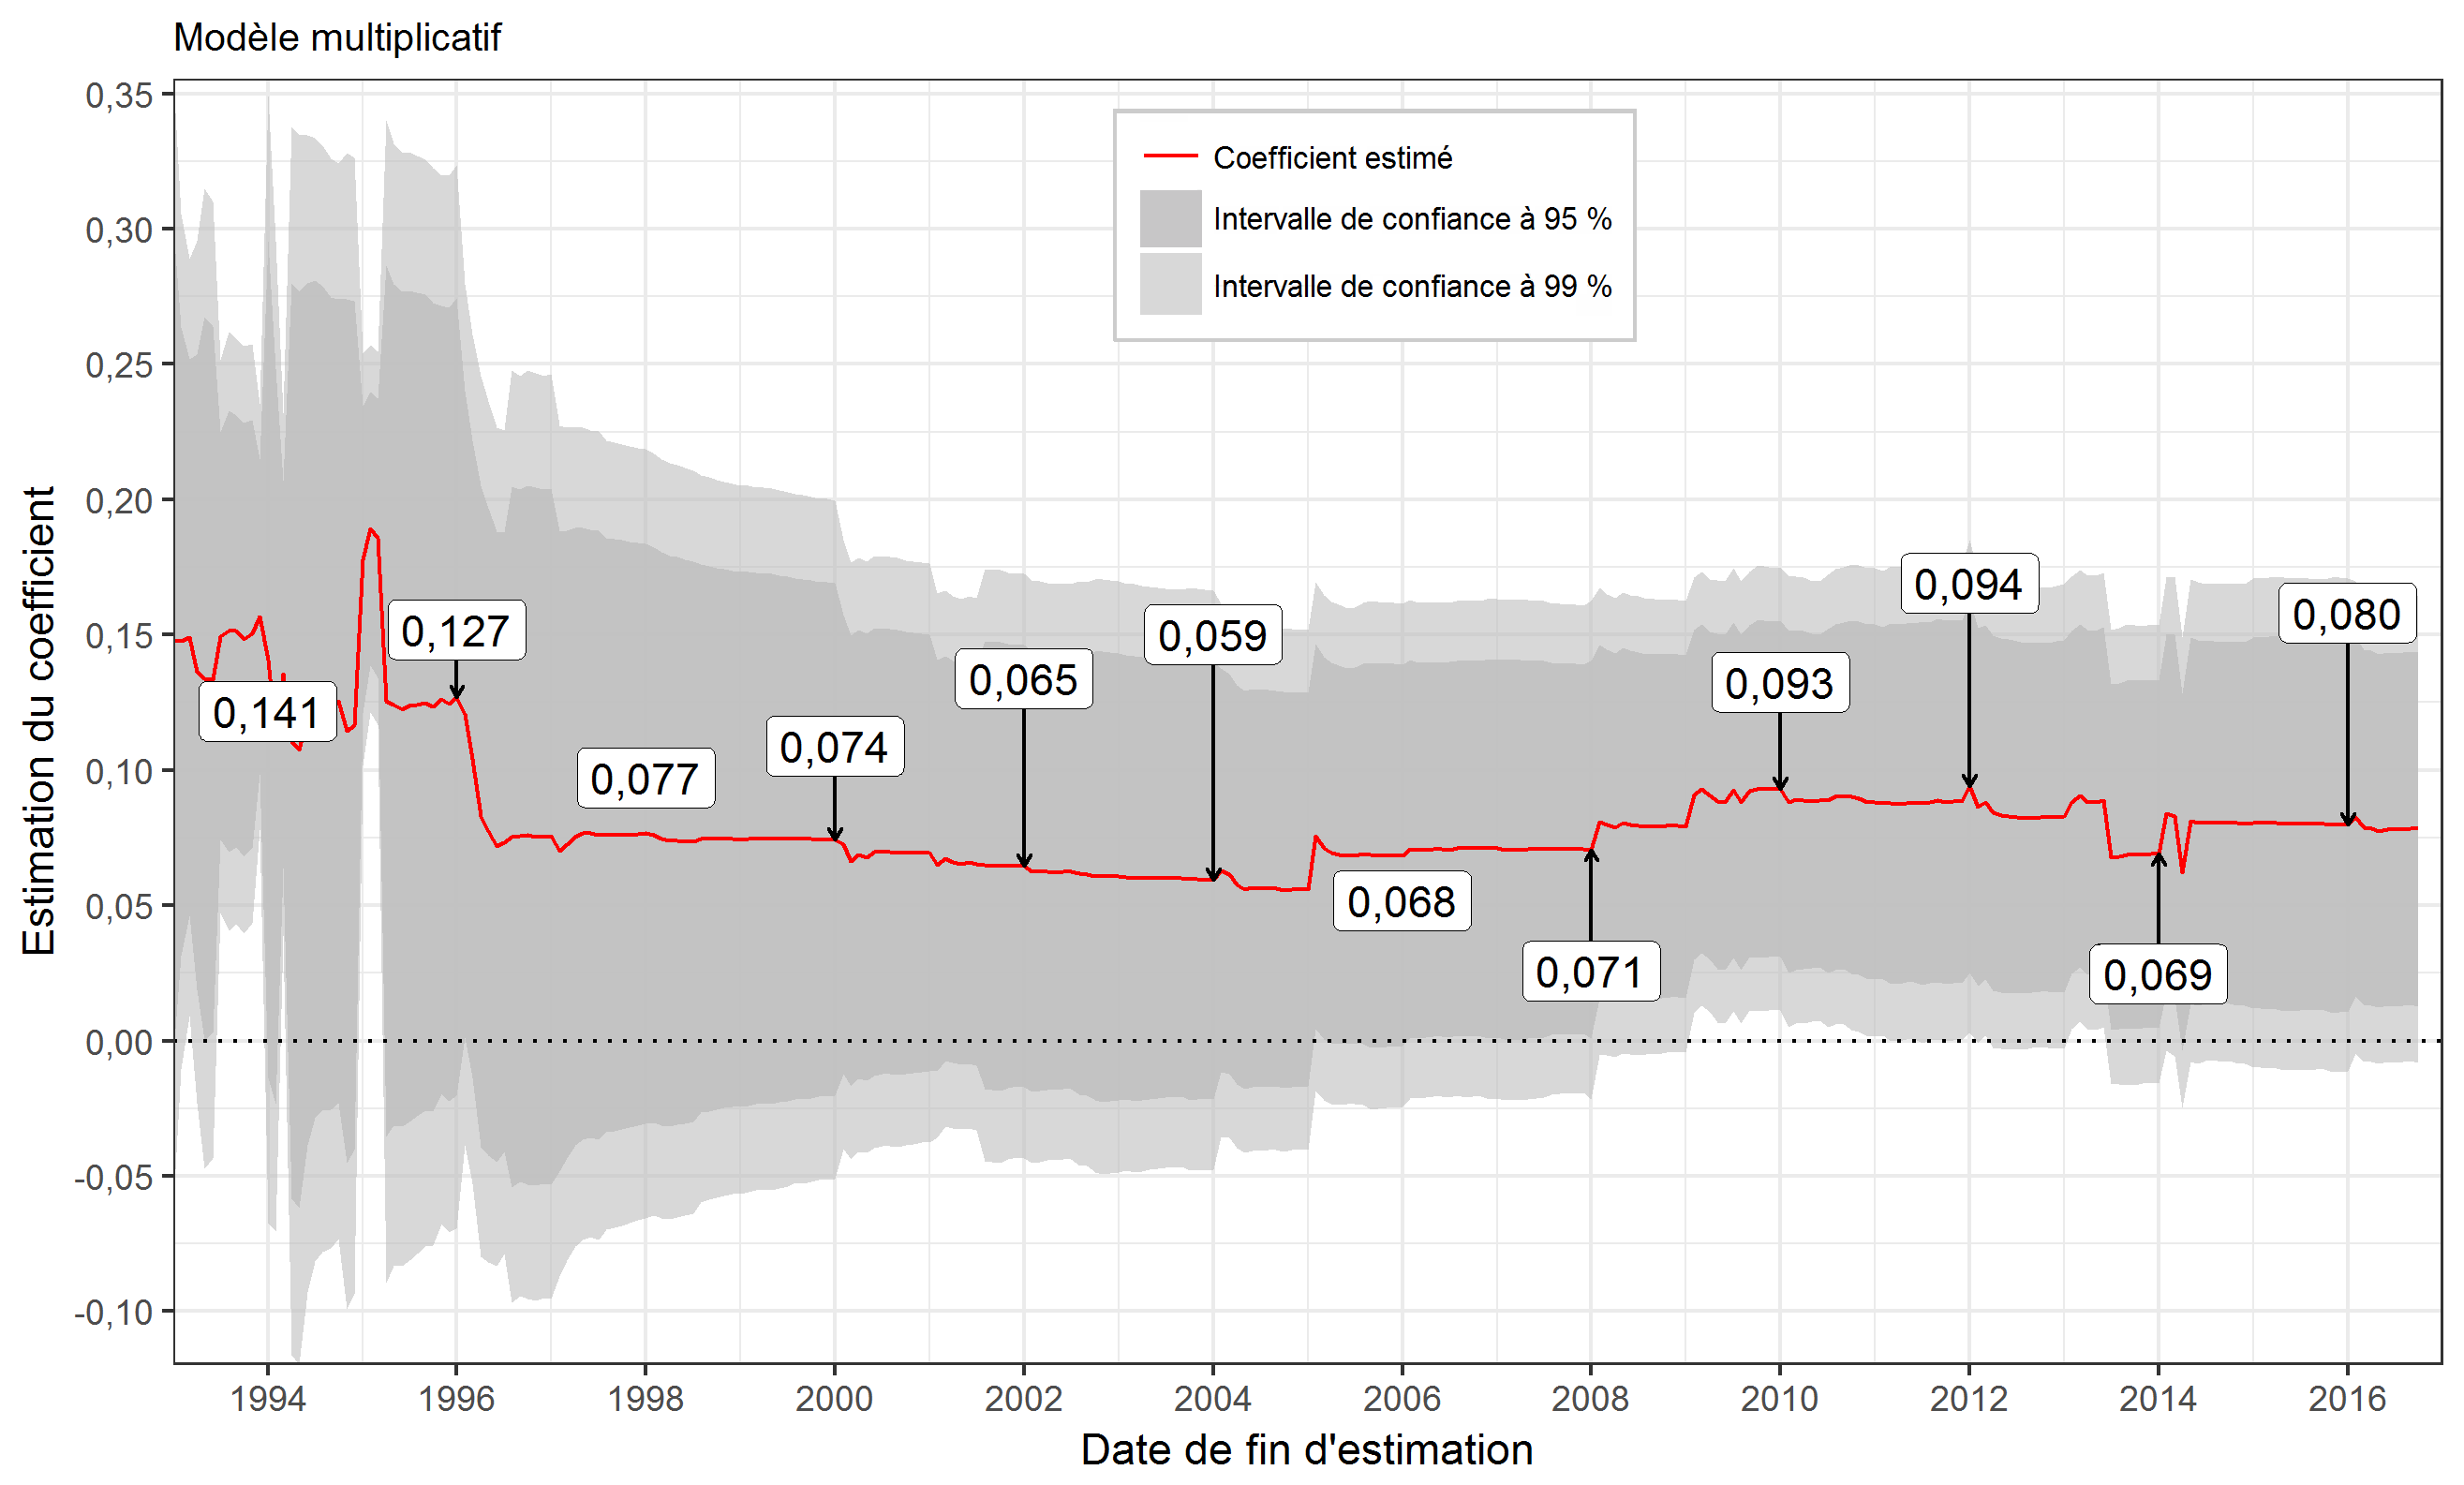
\includegraphics[width = \textwidth]{img/LYexemple2.png}

\end{frame}

\subsection{Résultats des simulations}\label{resultats-des-simulations}

\begin{frame}{Une convergence plutôt lente\ldots{}}

\centering
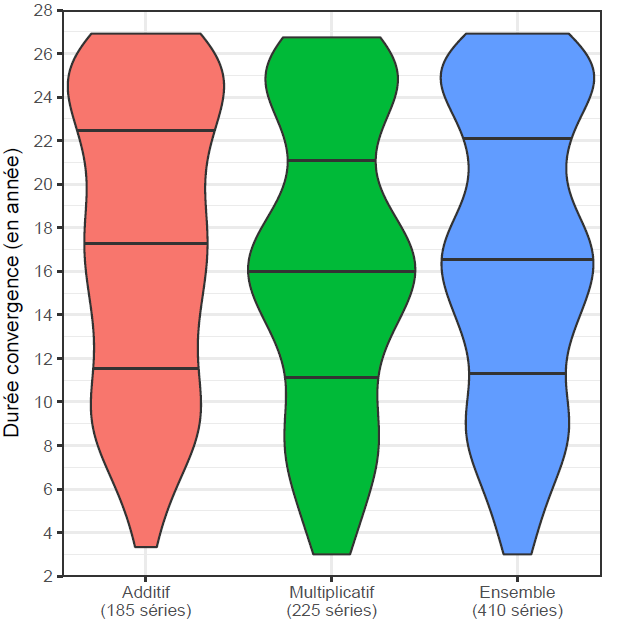
\includegraphics[height = 0.9\textheight]{img/LYconvergence.png}

\end{frame}

\begin{frame}{\ldots{} Vers une valeur pas toujours cohérente}

\centering
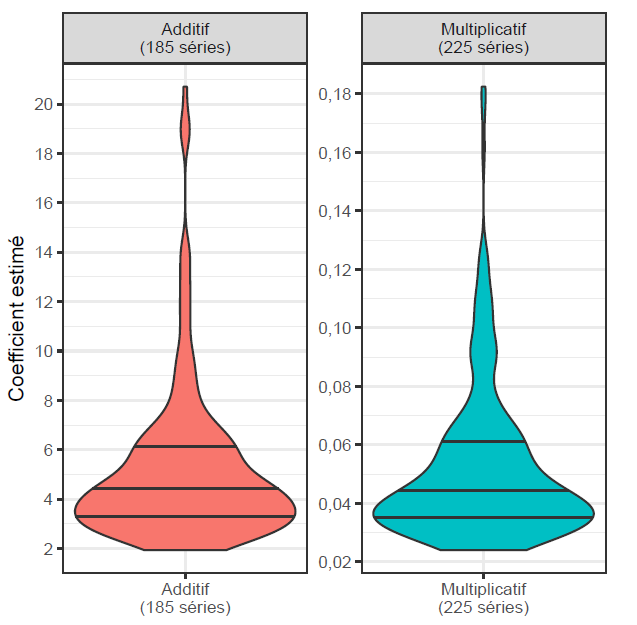
\includegraphics[height = 0.9\textheight]{img/LYvaleur.png}

\end{frame}

\begin{frame}{Comparaison des deux méthodes de correction}

\begin{figure}
\centering
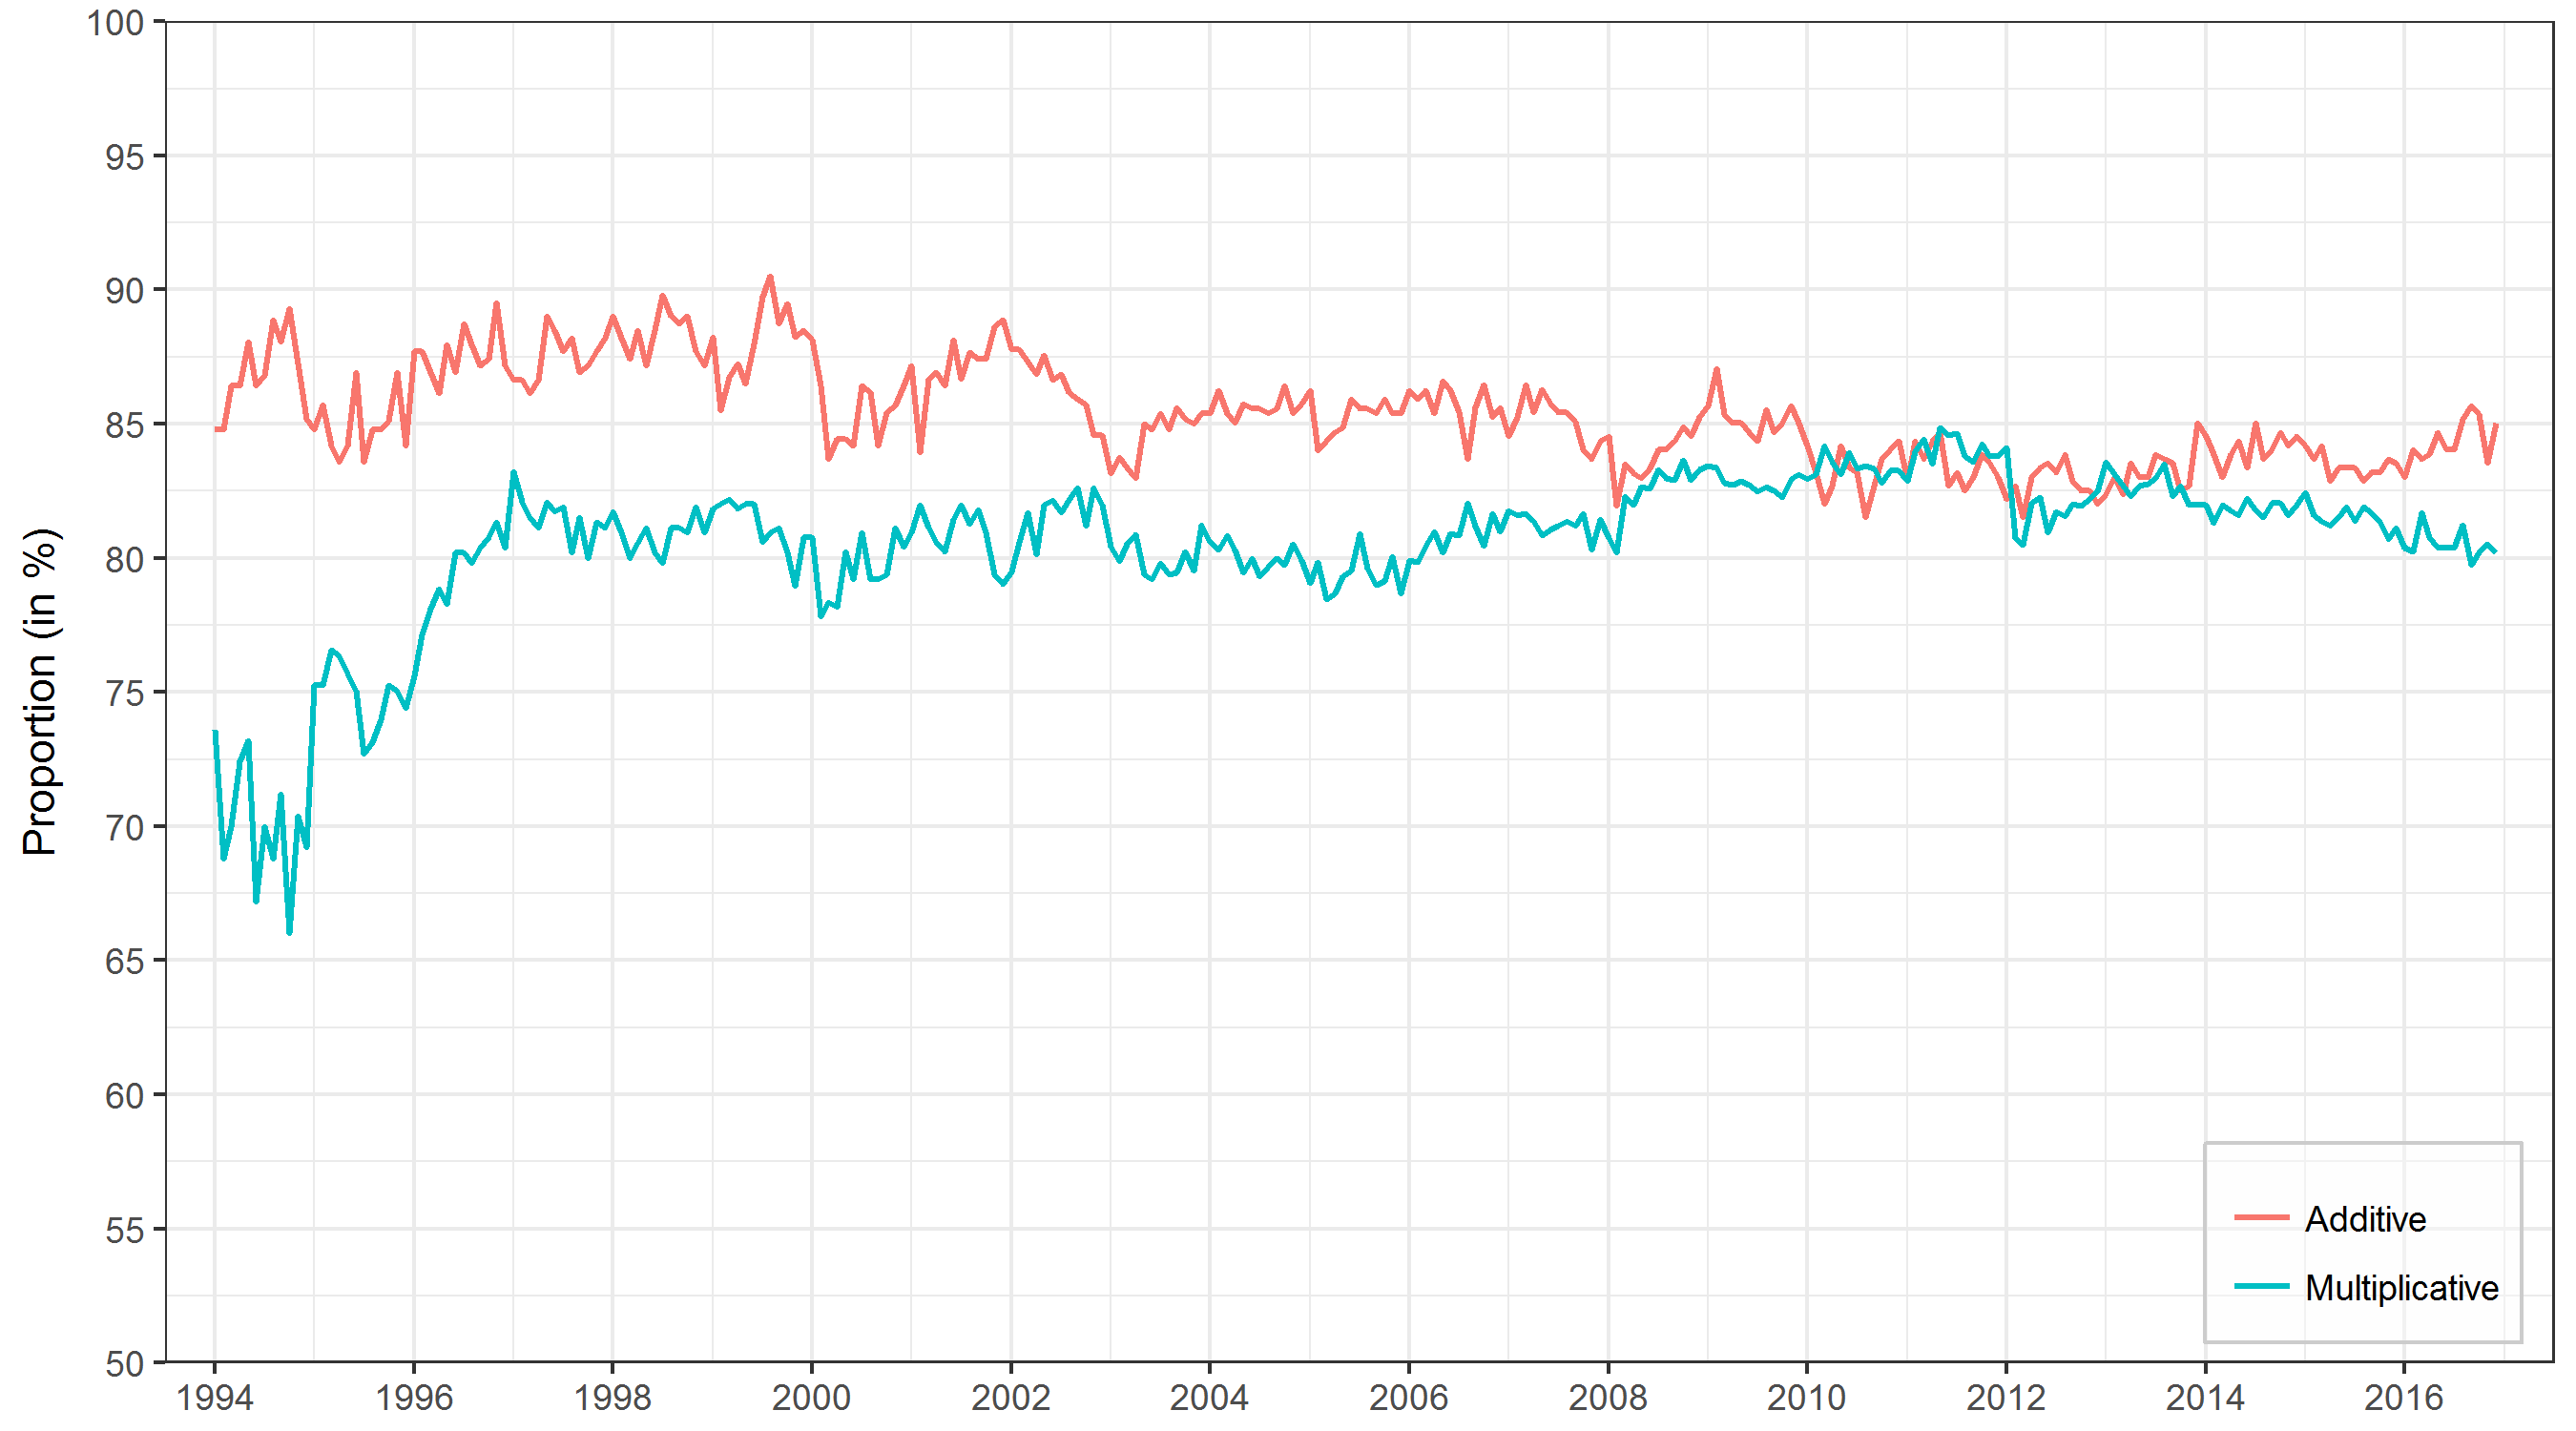
\includegraphics[width = \textwidth]{img/LYaicc.png}
\caption{Pourcentage des séries pour lesquelles l'AICC de la méthode 2 (pré-ajustement du LY) est inférieur à l'AICC méthode 1 (régresseur LY)}
\end{figure}

\end{frame}

\section{Correction des ruptures}\label{correction-des-ruptures}

\subsection{Les différentes ruptures
étudiées}\label{les-differentes-ruptures-etudiees}

\begin{frame}{Les principaux types d'\emph{outliers}}

\smallskip

\begin{columns}
\begin{column}{0.6\textwidth}
\textbf{Point atypique}

\emph{Additive outlier} (AO)
\end{column}
\begin{column}{0.3\textwidth}
% Created by tikzDevice version 0.10.1 on 2017-12-13 18:19:58
% !TEX encoding = UTF-8 Unicode
\begin{tikzpicture}[x=1pt,y=1pt]
\definecolor{fillColor}{RGB}{255,255,255}
\path[use as bounding box,fill=fillColor,fill opacity=0.00] (0,0) rectangle ( 93.95, 43.36);
\begin{scope}
\path[clip] (  0.00,  0.00) rectangle ( 93.95, 43.36);
\definecolor{drawColor}{RGB}{0,0,0}

\path[draw=drawColor,line width= 0.4pt,line join=round,line cap=round] (  3.48,  1.61) --
	(  4.40,  1.61) --
	(  5.31,  1.61) --
	(  6.23,  1.61) --
	(  7.14,  1.61) --
	(  8.06,  1.61) --
	(  8.97,  1.61) --
	(  9.89,  1.61) --
	( 10.81,  1.61) --
	( 11.72,  1.61) --
	( 12.64,  1.61) --
	( 13.55,  1.61) --
	( 14.47,  1.61) --
	( 15.38,  1.61) --
	( 16.30,  1.61) --
	( 17.22,  1.61) --
	( 18.13,  1.61) --
	( 19.05,  1.61) --
	( 19.96,  1.61) --
	( 20.88,  1.61) --
	( 21.79,  1.61) --
	( 22.71,  1.61) --
	( 23.63,  1.61) --
	( 24.54,  1.61) --
	( 25.46,  1.61) --
	( 26.37,  1.61) --
	( 27.29,  1.61) --
	( 28.20,  1.61) --
	( 29.12,  1.61) --
	( 30.04,  1.61) --
	( 30.95,  1.61) --
	( 31.87,  1.61) --
	( 32.78,  1.61) --
	( 33.70,  1.61) --
	( 34.61,  1.61) --
	( 35.53,  1.61) --
	( 36.44,  1.61) --
	( 37.36,  1.61) --
	( 38.28,  1.61) --
	( 39.19,  1.61) --
	( 40.11,  1.61) --
	( 41.02,  1.61) --
	( 41.94,  1.61) --
	( 42.85,  1.61) --
	( 43.77,  1.61) --
	( 44.69,  1.61) --
	( 45.60,  1.61) --
	( 46.52,  1.61) --
	( 47.43, 41.76) --
	( 48.35,  1.61) --
	( 49.26,  1.61) --
	( 50.18,  1.61) --
	( 51.10,  1.61) --
	( 52.01,  1.61) --
	( 52.93,  1.61) --
	( 53.84,  1.61) --
	( 54.76,  1.61) --
	( 55.67,  1.61) --
	( 56.59,  1.61) --
	( 57.51,  1.61) --
	( 58.42,  1.61) --
	( 59.34,  1.61) --
	( 60.25,  1.61) --
	( 61.17,  1.61) --
	( 62.08,  1.61) --
	( 63.00,  1.61) --
	( 63.92,  1.61) --
	( 64.83,  1.61) --
	( 65.75,  1.61) --
	( 66.66,  1.61) --
	( 67.58,  1.61) --
	( 68.49,  1.61) --
	( 69.41,  1.61) --
	( 70.33,  1.61) --
	( 71.24,  1.61) --
	( 72.16,  1.61) --
	( 73.07,  1.61) --
	( 73.99,  1.61) --
	( 74.90,  1.61) --
	( 75.82,  1.61) --
	( 76.74,  1.61) --
	( 77.65,  1.61) --
	( 78.57,  1.61) --
	( 79.48,  1.61) --
	( 80.40,  1.61) --
	( 81.31,  1.61) --
	( 82.23,  1.61) --
	( 83.15,  1.61) --
	( 84.06,  1.61) --
	( 84.98,  1.61) --
	( 85.89,  1.61) --
	( 86.81,  1.61) --
	( 87.72,  1.61) --
	( 88.64,  1.61) --
	( 89.56,  1.61) --
	( 90.47,  1.61);
\end{scope}
\end{tikzpicture}

\end{column}
\end{columns}

\begin{columns}
\begin{column}{0.6\textwidth}
\textbf{Changement de niveau}

\emph{Level Shift} (LS)
\end{column}
\begin{column}{0.3\textwidth}
% Created by tikzDevice version 0.10.1 on 2017-12-13 18:19:58
% !TEX encoding = UTF-8 Unicode
\begin{tikzpicture}[x=1pt,y=1pt]
\definecolor{fillColor}{RGB}{255,255,255}
\path[use as bounding box,fill=fillColor,fill opacity=0.00] (0,0) rectangle ( 93.95, 43.36);
\begin{scope}
\path[clip] (  0.00,  0.00) rectangle ( 93.95, 43.36);
\definecolor{drawColor}{RGB}{0,0,0}

\path[draw=drawColor,line width= 0.4pt,line join=round,line cap=round] (  3.48,  1.61) --
	(  4.40,  1.61) --
	(  5.31,  1.61) --
	(  6.23,  1.61) --
	(  7.14,  1.61) --
	(  8.06,  1.61) --
	(  8.97,  1.61) --
	(  9.89,  1.61) --
	( 10.81,  1.61) --
	( 11.72,  1.61) --
	( 12.64,  1.61) --
	( 13.55,  1.61) --
	( 14.47,  1.61) --
	( 15.38,  1.61) --
	( 16.30,  1.61) --
	( 17.22,  1.61) --
	( 18.13,  1.61) --
	( 19.05,  1.61) --
	( 19.96,  1.61) --
	( 20.88,  1.61) --
	( 21.79,  1.61) --
	( 22.71,  1.61) --
	( 23.63,  1.61) --
	( 24.54,  1.61) --
	( 25.46,  1.61) --
	( 26.37,  1.61) --
	( 27.29,  1.61) --
	( 28.20,  1.61) --
	( 29.12,  1.61) --
	( 30.04,  1.61) --
	( 30.95,  1.61) --
	( 31.87,  1.61) --
	( 32.78,  1.61) --
	( 33.70,  1.61) --
	( 34.61,  1.61) --
	( 35.53,  1.61) --
	( 36.44,  1.61) --
	( 37.36,  1.61) --
	( 38.28,  1.61) --
	( 39.19,  1.61) --
	( 40.11,  1.61) --
	( 41.02,  1.61) --
	( 41.94,  1.61) --
	( 42.85,  1.61) --
	( 43.77,  1.61) --
	( 44.69,  1.61) --
	( 45.60,  1.61) --
	( 46.52,  1.61) --
	( 47.43, 41.76) --
	( 48.35, 41.76) --
	( 49.26, 41.76) --
	( 50.18, 41.76) --
	( 51.10, 41.76) --
	( 52.01, 41.76) --
	( 52.93, 41.76) --
	( 53.84, 41.76) --
	( 54.76, 41.76) --
	( 55.67, 41.76) --
	( 56.59, 41.76) --
	( 57.51, 41.76) --
	( 58.42, 41.76) --
	( 59.34, 41.76) --
	( 60.25, 41.76) --
	( 61.17, 41.76) --
	( 62.08, 41.76) --
	( 63.00, 41.76) --
	( 63.92, 41.76) --
	( 64.83, 41.76) --
	( 65.75, 41.76) --
	( 66.66, 41.76) --
	( 67.58, 41.76) --
	( 68.49, 41.76) --
	( 69.41, 41.76) --
	( 70.33, 41.76) --
	( 71.24, 41.76) --
	( 72.16, 41.76) --
	( 73.07, 41.76) --
	( 73.99, 41.76) --
	( 74.90, 41.76) --
	( 75.82, 41.76) --
	( 76.74, 41.76) --
	( 77.65, 41.76) --
	( 78.57, 41.76) --
	( 79.48, 41.76) --
	( 80.40, 41.76) --
	( 81.31, 41.76) --
	( 82.23, 41.76) --
	( 83.15, 41.76) --
	( 84.06, 41.76) --
	( 84.98, 41.76) --
	( 85.89, 41.76) --
	( 86.81, 41.76) --
	( 87.72, 41.76) --
	( 88.64, 41.76) --
	( 89.56, 41.76) --
	( 90.47, 41.76);
\end{scope}
\end{tikzpicture}

\end{column}
\end{columns}

\begin{columns}
\begin{column}{0.6\textwidth}
\textbf{Rupture dans la composante saisonnière}

\emph{Seasonal Outlier} (SO) 
\end{column}
\begin{column}{0.3\textwidth}
% Created by tikzDevice version 0.10.1.2 on 2018-06-06 11:20:40
% !TEX encoding = UTF-8 Unicode
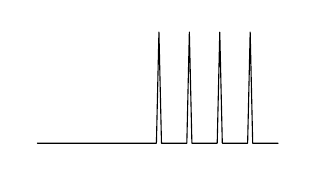
\begin{tikzpicture}[x=1pt,y=1pt]
\definecolor{fillColor}{RGB}{255,255,255}
\path[use as bounding box,fill=fillColor,fill opacity=0.00] (0,0) rectangle ( 93.95, 43.36);
\begin{scope}
\path[clip] (  0.00,  0.00) rectangle ( 93.95, 43.36);
\definecolor{drawColor}{RGB}{0,0,0}

\path[draw=drawColor,line width= 0.4pt,line join=round,line cap=round] (  3.48,  1.61) --
	(  4.40,  1.61) --
	(  5.31,  1.61) --
	(  6.23,  1.61) --
	(  7.14,  1.61) --
	(  8.06,  1.61) --
	(  8.97,  1.61) --
	(  9.89,  1.61) --
	( 10.81,  1.61) --
	( 11.72,  1.61) --
	( 12.64,  1.61) --
	( 13.55,  1.61) --
	( 14.47,  1.61) --
	( 15.38,  1.61) --
	( 16.30,  1.61) --
	( 17.22,  1.61) --
	( 18.13,  1.61) --
	( 19.05,  1.61) --
	( 19.96,  1.61) --
	( 20.88,  1.61) --
	( 21.79,  1.61) --
	( 22.71,  1.61) --
	( 23.63,  1.61) --
	( 24.54,  1.61) --
	( 25.46,  1.61) --
	( 26.37,  1.61) --
	( 27.29,  1.61) --
	( 28.20,  1.61) --
	( 29.12,  1.61) --
	( 30.04,  1.61) --
	( 30.95,  1.61) --
	( 31.87,  1.61) --
	( 32.78,  1.61) --
	( 33.70,  1.61) --
	( 34.61,  1.61) --
	( 35.53,  1.61) --
	( 36.44,  1.61) --
	( 37.36,  1.61) --
	( 38.28,  1.61) --
	( 39.19,  1.61) --
	( 40.11,  1.61) --
	( 41.02,  1.61) --
	( 41.94,  1.61) --
	( 42.85,  1.61) --
	( 43.77,  1.61) --
	( 44.69,  1.61) --
	( 45.60,  1.61) --
	( 46.52,  1.61) --
	( 47.43, 41.76) --
	( 48.35,  1.61) --
	( 49.26,  1.61) --
	( 50.18,  1.61) --
	( 51.10,  1.61) --
	( 52.01,  1.61) --
	( 52.93,  1.61) --
	( 53.84,  1.61) --
	( 54.76,  1.61) --
	( 55.67,  1.61) --
	( 56.59,  1.61) --
	( 57.51,  1.61) --
	( 58.42, 41.76) --
	( 59.34,  1.61) --
	( 60.25,  1.61) --
	( 61.17,  1.61) --
	( 62.08,  1.61) --
	( 63.00,  1.61) --
	( 63.92,  1.61) --
	( 64.83,  1.61) --
	( 65.75,  1.61) --
	( 66.66,  1.61) --
	( 67.58,  1.61) --
	( 68.49,  1.61) --
	( 69.41, 41.76) --
	( 70.33,  1.61) --
	( 71.24,  1.61) --
	( 72.16,  1.61) --
	( 73.07,  1.61) --
	( 73.99,  1.61) --
	( 74.90,  1.61) --
	( 75.82,  1.61) --
	( 76.74,  1.61) --
	( 77.65,  1.61) --
	( 78.57,  1.61) --
	( 79.48,  1.61) --
	( 80.40, 41.76) --
	( 81.31,  1.61) --
	( 82.23,  1.61) --
	( 83.15,  1.61) --
	( 84.06,  1.61) --
	( 84.98,  1.61) --
	( 85.89,  1.61) --
	( 86.81,  1.61) --
	( 87.72,  1.61) --
	( 88.64,  1.61) --
	( 89.56,  1.61) --
	( 90.47,  1.61);
\end{scope}
\end{tikzpicture}

\end{column}
\end{columns}

\begin{columns}
\begin{column}{0.6\textwidth}
\textbf{Changement transitoire de niveau}

\emph{Transitory Change} (TC) 
\end{column}
\begin{column}{0.3\textwidth}
% Created by tikzDevice version 0.10.1 on 2017-12-13 18:19:58
% !TEX encoding = UTF-8 Unicode
\begin{tikzpicture}[x=1pt,y=1pt]
\definecolor{fillColor}{RGB}{255,255,255}
\path[use as bounding box,fill=fillColor,fill opacity=0.00] (0,0) rectangle ( 93.95, 43.36);
\begin{scope}
\path[clip] (  0.00,  0.00) rectangle ( 93.95, 43.36);
\definecolor{drawColor}{RGB}{0,0,0}

\path[draw=drawColor,line width= 0.4pt,line join=round,line cap=round] (  3.48,  1.61) --
	(  4.40,  1.61) --
	(  5.31,  1.61) --
	(  6.23,  1.61) --
	(  7.14,  1.61) --
	(  8.06,  1.61) --
	(  8.97,  1.61) --
	(  9.89,  1.61) --
	( 10.81,  1.61) --
	( 11.72,  1.61) --
	( 12.64,  1.61) --
	( 13.55,  1.61) --
	( 14.47,  1.61) --
	( 15.38,  1.61) --
	( 16.30,  1.61) --
	( 17.22,  1.61) --
	( 18.13,  1.61) --
	( 19.05,  1.61) --
	( 19.96,  1.61) --
	( 20.88,  1.61) --
	( 21.79,  1.61) --
	( 22.71,  1.61) --
	( 23.63,  1.61) --
	( 24.54,  1.61) --
	( 25.46,  1.61) --
	( 26.37,  1.61) --
	( 27.29,  1.61) --
	( 28.20,  1.61) --
	( 29.12,  1.61) --
	( 30.04,  1.61) --
	( 30.95,  1.61) --
	( 31.87,  1.61) --
	( 32.78,  1.61) --
	( 33.70,  1.61) --
	( 34.61,  1.61) --
	( 35.53,  1.61) --
	( 36.44,  1.61) --
	( 37.36,  1.61) --
	( 38.28,  1.61) --
	( 39.19,  1.61) --
	( 40.11,  1.61) --
	( 41.02,  1.61) --
	( 41.94,  1.61) --
	( 42.85,  1.61) --
	( 43.77,  1.61) --
	( 44.69,  1.61) --
	( 45.60,  1.61) --
	( 46.52,  1.61) --
	( 47.43, 41.76) --
	( 48.35, 29.71) --
	( 49.26, 21.28) --
	( 50.18, 15.38) --
	( 51.10, 11.25) --
	( 52.01,  8.35) --
	( 52.93,  6.33) --
	( 53.84,  4.91) --
	( 54.76,  3.92) --
	( 55.67,  3.23) --
	( 56.59,  2.74) --
	( 57.51,  2.40) --
	( 58.42,  2.16) --
	( 59.34,  2.00) --
	( 60.25,  1.88) --
	( 61.17,  1.80) --
	( 62.08,  1.74) --
	( 63.00,  1.70) --
	( 63.92,  1.67) --
	( 64.83,  1.65) --
	( 65.75,  1.64) --
	( 66.66,  1.63) --
	( 67.58,  1.62) --
	( 68.49,  1.62) --
	( 69.41,  1.61) --
	( 70.33,  1.61) --
	( 71.24,  1.61) --
	( 72.16,  1.61) --
	( 73.07,  1.61) --
	( 73.99,  1.61) --
	( 74.90,  1.61) --
	( 75.82,  1.61) --
	( 76.74,  1.61) --
	( 77.65,  1.61) --
	( 78.57,  1.61) --
	( 79.48,  1.61) --
	( 80.40,  1.61) --
	( 81.31,  1.61) --
	( 82.23,  1.61) --
	( 83.15,  1.61) --
	( 84.06,  1.61) --
	( 84.98,  1.61) --
	( 85.89,  1.61) --
	( 86.81,  1.61) --
	( 87.72,  1.61) --
	( 88.64,  1.61) --
	( 89.56,  1.61) --
	( 90.47,  1.61);
\end{scope}
\end{tikzpicture}

\end{column}
\end{columns}

\end{frame}

\subsection{Méthodologie de l'étude}\label{methodologie-de-letude-1}

\begin{frame}{Méthodologie utilisée}

Sur les IPI européens :

\begin{enumerate}
\def\labelenumi{\arabic{enumi}.}
\item
  \highlightbf{identification} et \highlightbf{estimation} du modèle sur
  13 ans
\item
  simulation d'une rupture 5 ans après la date de début de niveau 10
  pour un modèle \highlightbf{additif}
\item
  estimation du coefficient de la rupture en figeant les estimations de
  tous les autres paramètres et la date de début d'estimation
\end{enumerate}

On considère qu'il y a convergence lorsque :
\[\left\lvert\frac{\text{valeur estimée}}{\text{dernière valeur estimée}}-1\right\rvert < 5\;\%\]

\end{frame}

\subsection{Exemple}\label{exemple}

\begin{frame}{Exemple d'un AO pour la série IPI IT-1413 (Fabrication de
vêtements de dessus)}

\centering

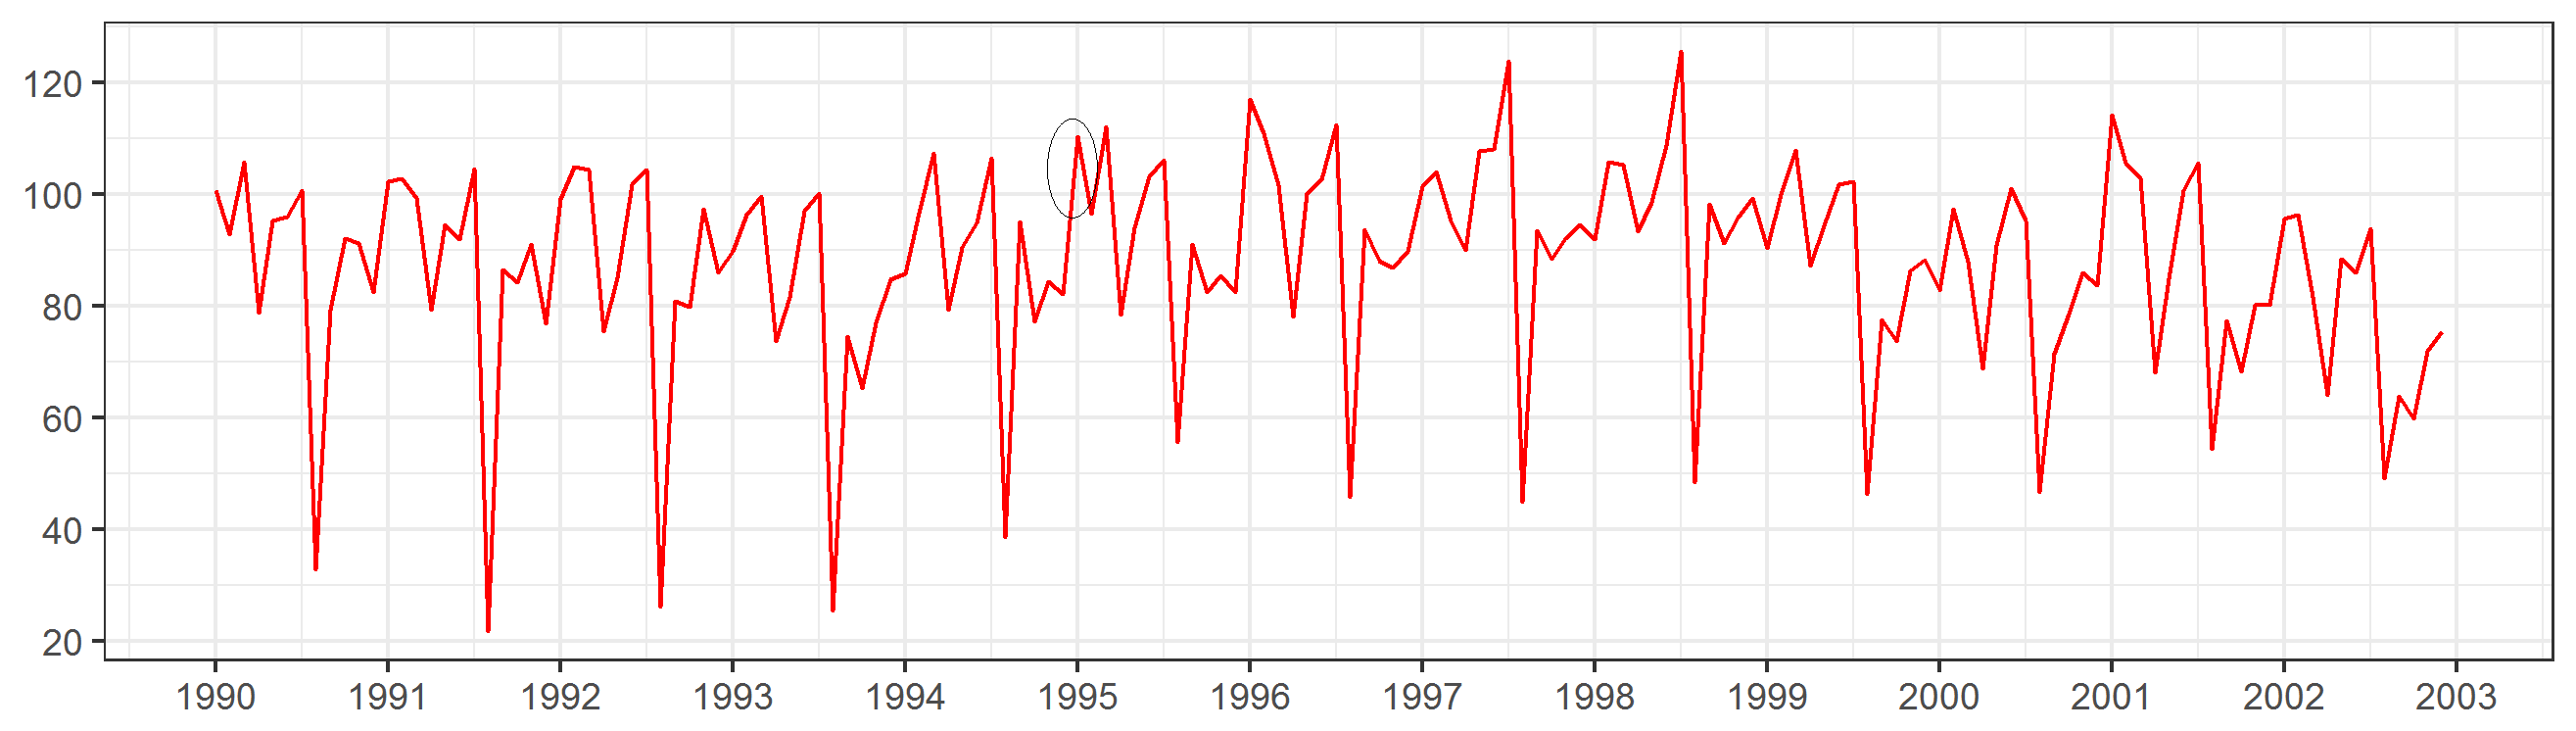
\includegraphics[width=0.95\textwidth]{img/AO_ipi_it1413_y.png}

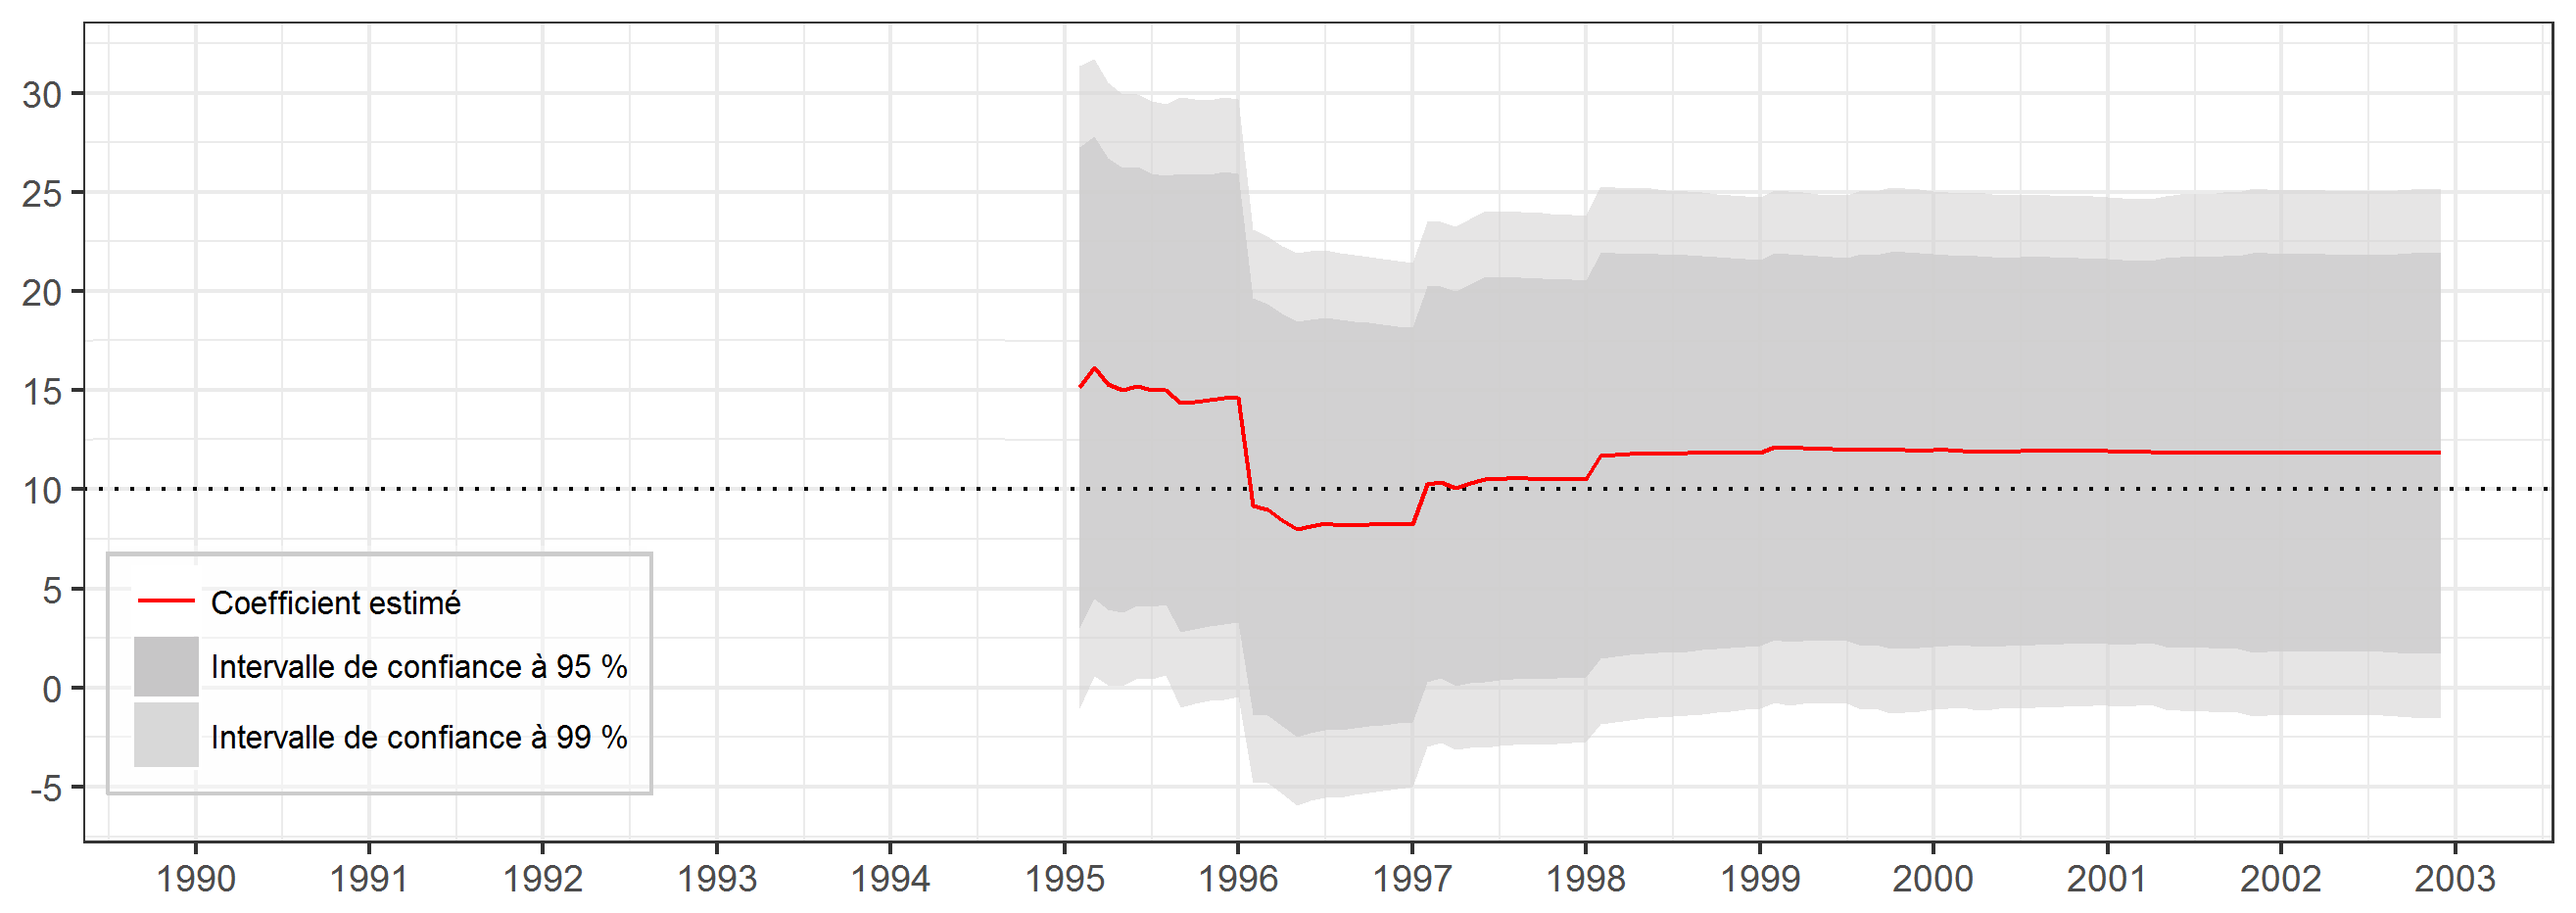
\includegraphics[width=0.95\textwidth]{img/AO_ipi_it1413_est.png}

\end{frame}

\subsection{Résultats des
simulations}\label{resultats-des-simulations-1}

\begin{frame}{Une convergence plutôt lente\ldots{}}

\centering
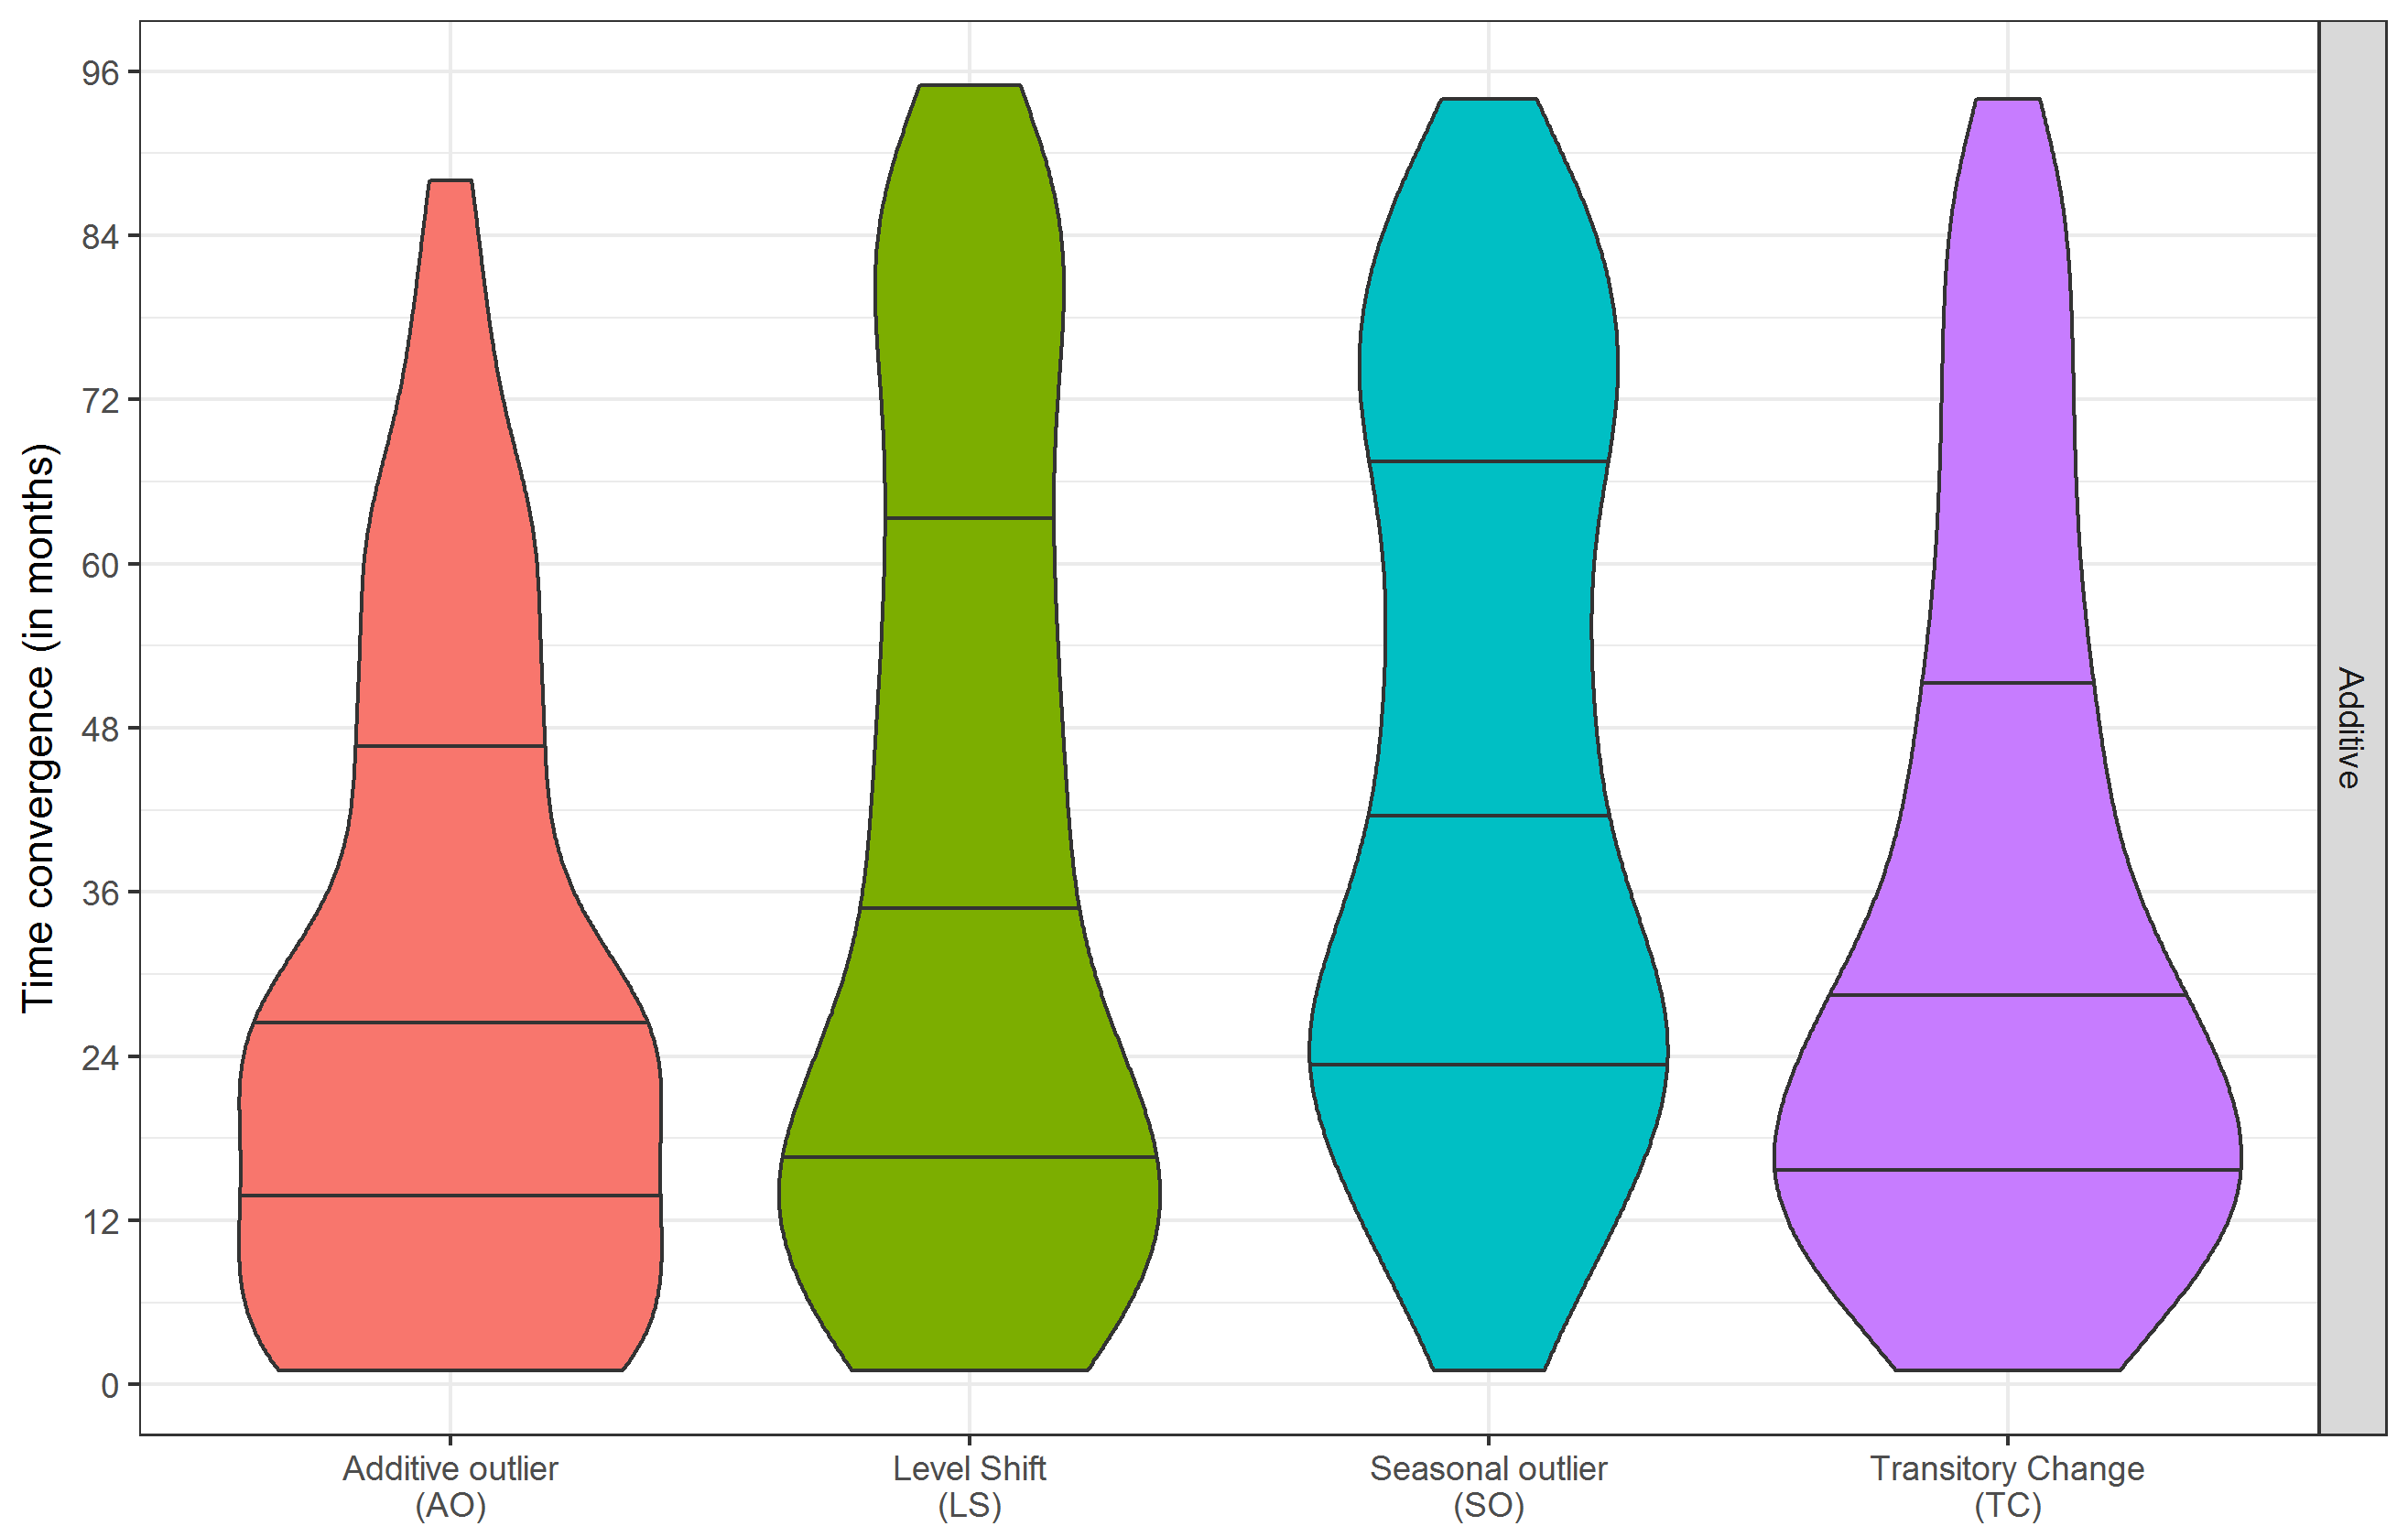
\includegraphics[width=1.00000\textwidth]{img/outliers_convergence_additif_5.png}\\

\end{frame}

\begin{frame}{\ldots{} Mais pas toujours vers la bonne valeur}

\centering

\begin{tabular}{lccccc}\toprule
  & Minimum & 25   \% & 50   \% & 75   \% & Maximum\\\midrule
\addlinespace[0.3em]\multicolumn{6}{l}{\textbf{Modèles additifs}}\\
\hspace{1em}Additive outlier (AO) & -73,4 & 8,0 & 11,0 & 14,4 & 45,9\\
\hspace{1em}Level Shift (LS) & -33,9 & 6,3 & 9,2 & 12,8 & 95,0\\
\hspace{1em}Seasonal outlier (SO) & -83,5 & 5,9 & 8,1 & 10,4 & 34,3\\
\hspace{1em}Transitory Change (TC) & -56,9 & 6,9 & 10,2 & 14,2 & 133,5\\\addlinespace[0.3em]
\bottomrule\end{tabular}

\end{frame}

\section{Identification du modèle
ARIMA}\label{identification-du-modele-arima}

\begin{frame}{Identification de deux modèles équivalents}

On reprend le même modèle de base sous deux formes différentes
mathématiquement équivalentes :

\begin{enumerate}
\def\labelenumi{\arabic{enumi}.}
\item
  Le régresseur \emph{leap year} intégré dans le système des régresseurs
  jours ouvrables
\item
  Le régresseur \emph{leap year} introduit comme régresseur externe
\end{enumerate}

\(\rightarrow\) étude du modèle automatique

\end{frame}

\begin{frame}{Modèles automatiques différents}

\centering
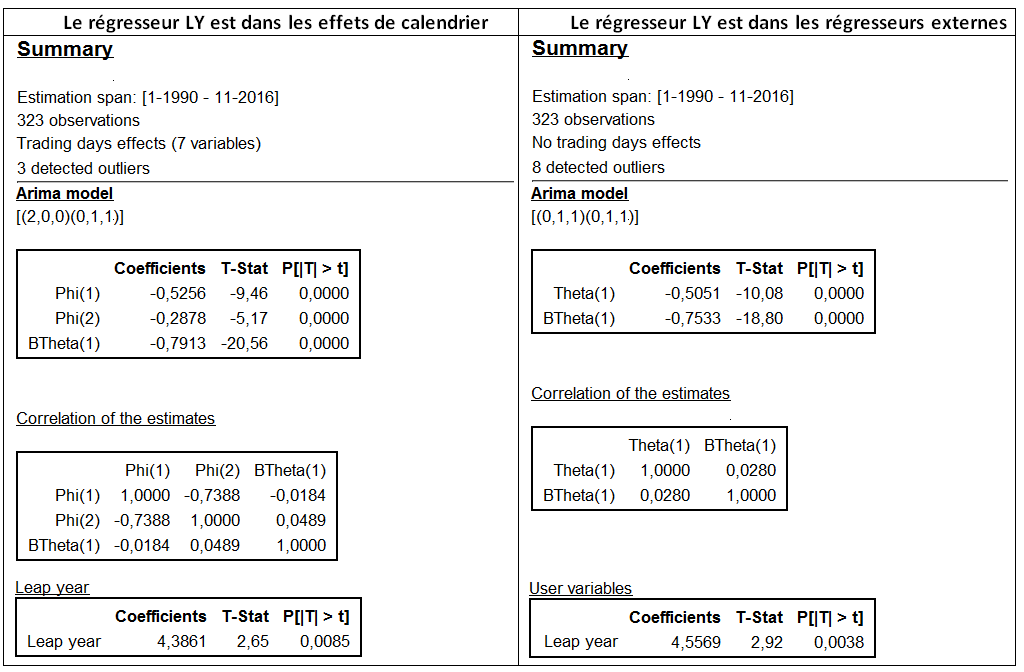
\includegraphics[width = \textwidth]{img/CholeskyRF241.png}

\end{frame}

\section{Conclusion et
recommandations}\label{conclusion-et-recommandations}

\begin{frame}{Conclusion et recommandations (1/2)}

\medskip

\bcinfo Simulations \highlightbfslide{1}{critiquables} et
\highlightbfslide{1}{améliorables} mais mettent en évidence la
\highlightbfslide{1}{potentielle instabilité} des modèles Reg-ARIMA
souvent utilisés comme boîtes noires

\medskip  \pause
\bcsmbh Instabilités ont un \highlightbfslide{2}{effet limité} sur la
CVS-CJO\dots \bcsmmh mais ont un effet sur l'histoire à
\highlightbfslide{2}{court terme} et sur les
\highlightbfslide{2}{révisions} !

\medskip  \pause
\bcattention Algorithmes automatiques des méthodes X-13ARIMA-SEATS et
TRAMO-SEATS très \highlightbfslide{3}{importants} et très
\highlightbfslide{3}{utiles}

\end{frame}

\begin{frame}{Conclusion et recommandations (2/2)}

Spécifier le modèle \highlightbf{au préalable} au niveau de la
\highlightbf{série} :

\begin{itemize}
\item
  baser les procédures de choix en s'appuyant sur un raisonnement
  d'abord économique (attention aux séries trop longues)
\item
  \bcinterdit ne pas utiliser les méthodes comme des boîtes
  noires\ldots{} \pause Sinon, vous serez comme ce statisticien
  qui\ldots{}
\end{itemize}

\end{frame}

\begin{frame}{Merci de votre attention}

\begin{quote}
« Il se sert des statistiques comme un ivrogne d'un réverbère : pour se soutenir et non pour s'éclairer. »
\end{quote}

Citation largement attribuée à Andrew Lang (1844-1912)

\addtocounter{framenumber}{-1}

\end{frame}

\end{document}
